%!TEX root = ../konzept.tex

\section{Datenmodell}

Aufgrund der verteilten Anwendung und der lokalen Speicherung von Daten müssen die einzelen Komponten untereinander die Daten austauschen. Dafür ist es nötig, dass jede Kompontene mit den Daten arbeiten kann.

Die lokale Anwendung für Mieter und Vermieter arbeitet dabei mit einer SQL Lite Datenbank und speichert die Informationen des Users, wie Vorname, Nachname oder das Geburtsdatum auf dem Smartphone. Grundsätzlich sollten nur soviele Informationen wie zur Identifikation des Anwenders notwendig sind, angabepflichtig sein. Zusätzlich zum \"Userprofil\", besteht die Möglichkeit als Vermieter Grundstücke anzulegen. Neben einer allgemeinen Grundstücks ID, die automatisch festgelegt wird und später beim Abgleich notwendig ist, geht es hierbei darum die Ausstattung zu präzisieren. 
Das könnten Aspekte wie Platzgröße, sanitäre Einrichtung oder sonstige Leistungen wie Internet oder Stromanschluss sein. Wichtig ist hierbei, dass diese Informationen später beim Matching verglichen werden. Daher sollten hier keine Freitexteingabe auftreten, sondern mit Auswahloptionen gearbeitet werden. Vorrangig wird hierbei mit Zahlen, Boolschen Werten und statischen Textwerten gearbeitet. Bei einer Reise erstellt der Mieter eine \"Mietanfrage\" und legt dort seine Ausstattung fest, die während der Anfrage versendet wird. Da die Datengröße einer Nachricht über GCM (nach aktuellem Informationsstand) nur 4 KByte beträgt, ist es nicht möglich, auf diesem Weg Bilder zu Mietobjekten zu übersenden. 
Die zweite Datenbank ist mit dem Server verbunden und beinhaltet eine Liste aller registrierten User mit ihren Devices, sowie die Zuordnung zu vorhandenen Mietobjekten. Auf sensible Daten soll hierbei bewusst verzichtet werden, damit im Falle eines Angriffes, keine Informationen zur Bankverbindung oder Mietobjekte öffentlich gemacht werden.

Folgende Abbildung \ref{fig:kommunikationsablauf} verdeutlicht diesen Kommunikationsablauf mit entsprechender Datenbankanbindung und zeigt mit welchen Datenbankschlüsseln mindesten gearbeitet werden soll.
Aufgrund der Datenaufteilung auf die unterschiedlichen Komponenten, ist ein einheitliches Datenbank bzw. ER Modell visuell nur schwer umzusetzen. Dieser Ansatz verdeutlicht die angedachten Entitäten mit vorhandenen Attributen.

\begin{figure}[H]
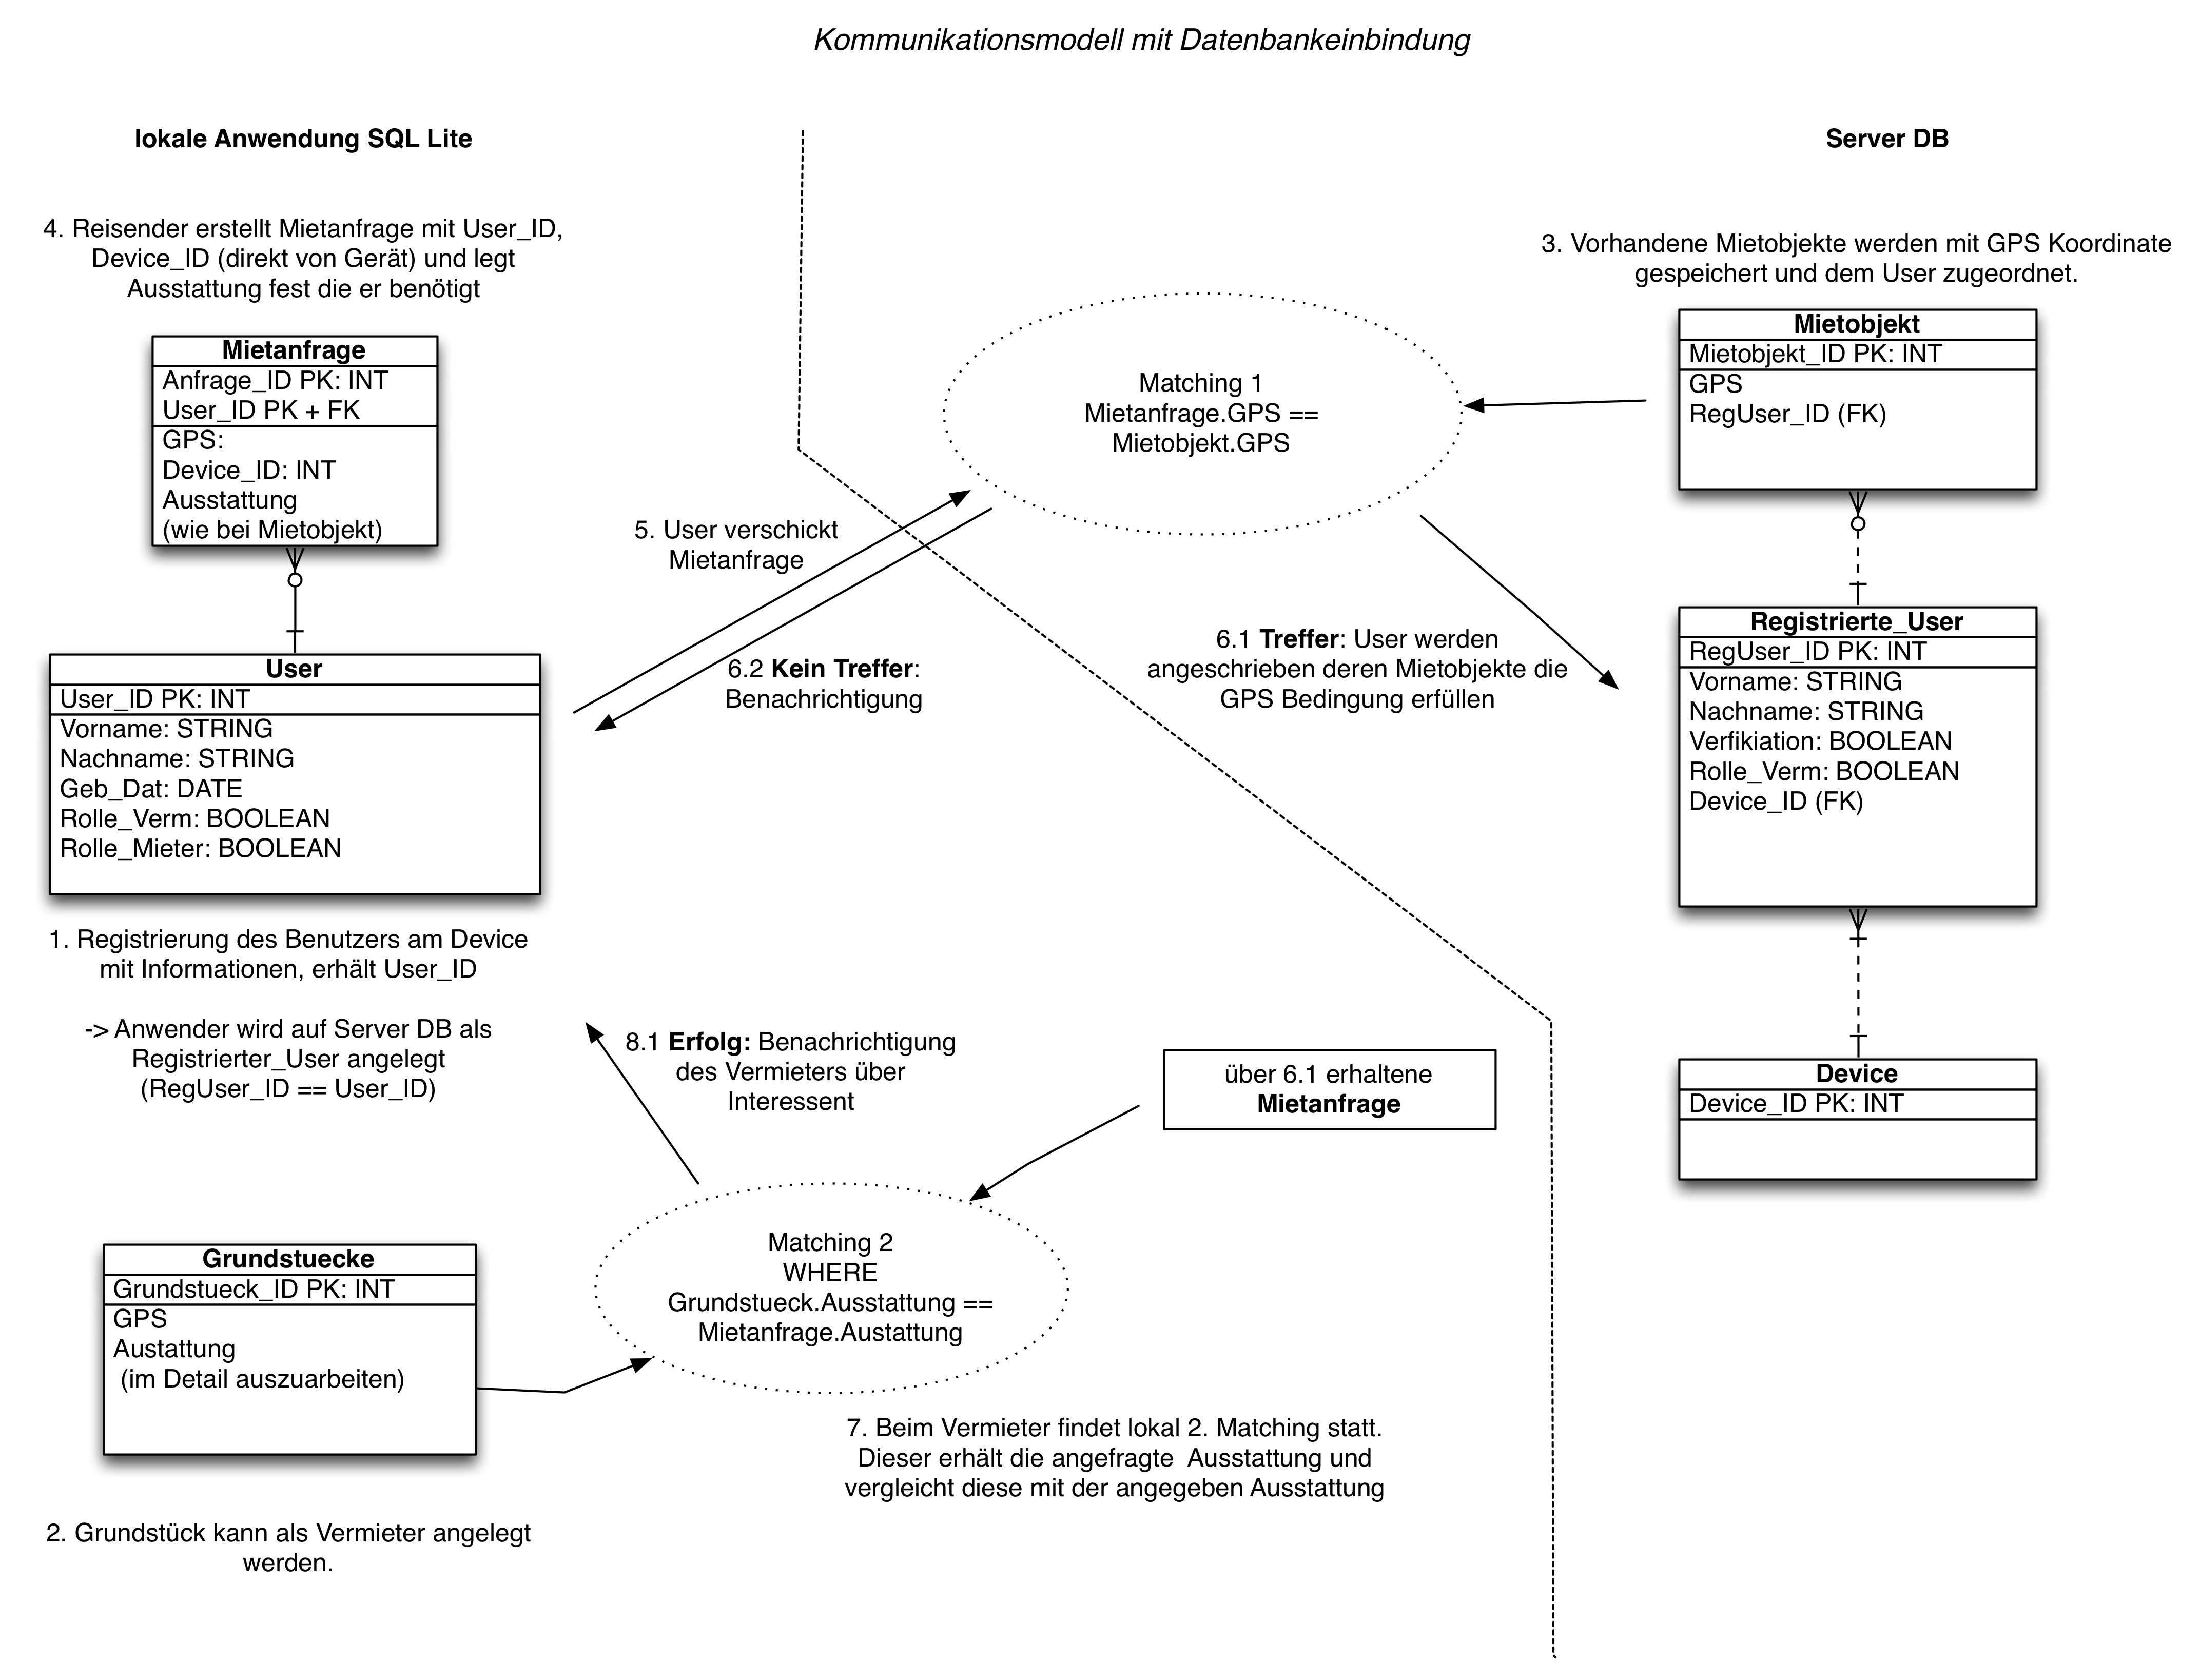
\includegraphics[width=1\textwidth]{./images/kommunikationsmodell_mit_datenbank.png}
\caption{Kommunikationsmodell mit Datenbankeinbindung}
\label{fig:kommunikationsablauf}
\end{figure}

Speziell in Hinblick auf das zweite Matching, ist es notwendig, die einzelnen Attribute zur Ausstattung vorzudefinieren. Ein erster Entwurf dazu zeigt sich in folgender Tabelle \ref{tab:ausstattungsattribute}.

Attribute die als notwendig erachtet werden, sind der Preisrahmen (price\_range) in welchem die Übernachtungskosten liegen sollten, die Gruppengröße, die Option ob Toiletten, Dusche, Bad und Storm vorhanden ist und ob Kinder gestattet werden. Diese Angaben sollten immer vorhanden sein. 
Zusätzliche Optionen beziehen sich auf die direkte Umgebung und sonstige Genehmigungen und Angebote von Seiten des Vermieters. Zusätzlich denkbar wäre noch eine Freitext Option für Kurzinformationen. Diese fließen jedoch nicht in den Matchingalgorithmus ein.


\begin{table}[H]
\caption{Attribute zur Ausstattung}
\centering
\begin{tabular}{|l|l|l|}
\hline
\ \textbf{Attributname}                         						 & \textbf{Datentyp} 					  & \textbf{Constraint} 					  \\ \hline
toilets\_available                                                   & boolean                                & not null                                  \\ \hline
bbq\_allowed                                                         & boolean                                & null                                      \\ \hline
internet\_available                                                  & boolean                                & null                                      \\ \hline
carparking\_possible                                                 & boolean                                & null                                      \\ \hline
children\_allowed                                                    & boolean                                & not null                                  \\ \hline
supermarket\_nearby                                                  & boolean                                & null                                      \\ \hline
public\_transport\_nearby 	  										 & boolean                                & null                                      \\ \hline
shower\_bath\_available                                              & boolean                                & not null                                  \\ \hline
water\_provided                                                      & boolean                                & null                                      \\ \hline
tents\_provided                                                      & boolean                                & null                                      \\ \hline
power\_provided                                                      & boolean                                & not null                                  \\ \hline
dogs\_allowed                                                        & boolean                                & null                                      \\ \hline
group\_size                                                          & number                                 & not null                                  \\ \hline
caravan\_parking\_possible  										 & boolean                                & null                                      \\ \hline
price\_range                                                         & number                                 & not null                                  \\ \hline
campfire\_allowed                                                    & boolean                                & null                                      \\ \hline
\end{tabular}
\label{tab:ausstattungsattribute}
\end{table}

Der Matchingalgorithmus sollte auf diesen Angaben aufbauen und sie je nach Relevanz unterschiedlich gewichten.
Die Gruppengröße muss unter der maximalen Kapazität des Grundstückes liegen und der Mietpreis sollte sich im Preisrahmen des Reisenden befinden. 
Die Angabe, ob Kinder erlaubt sind, wird als dritter maßgeblicher Faktor ausgelegt, da sich daran keine Kompromisse für den Reisenden finden lassen.
Anhand der weiteren Pflichtangaben wird die Relevanz bedeutend erhöht und verringert. Die zusätzlichen Faktoren beeinflussen den Matchingquotienten ebenfalls, sollten in ihrer Gewichtung aber eine geringere Stärke aufweisen, damit die wesentlichen Aspekte im Fokus liegen und kein Luxusfaktor, wie offenes Campfeuer, die Anfrage herausfiltert.
